\documentclass[12pt]{article}
\usepackage{titlesec}
\usepackage{float}
\usepackage{graphicx}

\usepackage{hyperref}
\hypersetup{
    colorlinks,
    citecolor=black,
    filecolor=black,
    linkcolor=black,
    urlcolor=black
}

\begin{document}

\title{Test Report for Content Management System} 
\author{Team: The Outsiders\\ Kirk Montour (montour)\\ Syed Gardezi (gardezsh)}
\date{\today}
  
\maketitle



\pagebreak

\tableofcontents

\pagebreak

\section{Revision History}
This section is used to record major changes to the document.
\begin{table}[H]
\centering
\caption{Revision History}
\begin{tabular}{|l|l|l|}
\hline
\textbf{Changes to the Document}                          & \textbf{Author}     & \textbf{Date}       \\ \hline
Initial draft of document                        & Kirk, Syed & 24-02-2017 \\ \hline
Conducted usability tests and documented results & Kirk       & 02-03-2017 \\ \hline
Conducted system tests and documented results    & Syed       & 03-03-2017 \\ \hline
Conducted performance tests and documented results    & Kirk, Syed & 10-03-2017 \\ \hline
\end{tabular}
\end{table}

\listoftables

\section{Introduction}
In this testing report we will be documenting the results for both
system tests and non-functional tests on the content management system.

\subsection{Acronyms}

\begin{table}[h]
\centering
\caption{Acronyms used}
\label{my-label}
\begin{tabular}{|l|l|}
\hline
UI  & User Interface            \\ \hline
CMS & Content Management System \\ \hline
\end{tabular}
\end{table}

\section{Usability Testing}

\subsection{Learnability}
Learnability is how easy it is for users to accomplish the usability tasks the first time they encounter the user interface (UI).\\
Learnability was very high for most tasks due to the similarity of the tasks with common web surfing tasks such as registering for websites and filling out forms, therefore only significant deviation from common web surfing tasks which increased learnability will be noted in the individual usability tasks.

\subsection{Efficiency}
Efficiency pertaining to usability testing is how fast can experienced users accomplish tasks. \\
Efficiency was very high for most tasks also due to the similarity of the tasks with common web surfing tasks as previously mentioned with Learnability. Since efficiency is related to experienced users and a content management system (CMS) targets non-technical users, efficiency will not be noted in the individual usability tasks.   

\subsection{Memorability}

Memorability is when users return to the usability task after not using it for a while and still remember how to do the usability task.\\
Memorability was very high for all tasks due to previous experience with registering for websites and filling out forms. Therefore, the Memorability aspects of the usability tasks will not be noted.

\subsection{Errors}
Errors are how many errors users make, how severe the errors are, and recoverability from errors.\\
Errors were negligible for the usability tasks due to the similarity of the usability tasks with common web surfing tasks. Errors will be reflected in the usability task completion time and will not be noted in individual usability tasks.

\subsection{User Satisfaction}
User satisfaction is how much did the user enjoy using the CMS.\\
User Satisfaction was very positive. As non-technical users, the idea of creating web pages with a word processor like editor and seeing the page they created displayed on the front-end created a “this is so cool” type of energy from the users.
\par
To test usability, learnability will be measured. A usability task will be completed 5 times with the task completion time recorded. 4 non-technical users and one technical user will execute the usability tasks 5 times each. A non-technical user is an ordinary web surfer with no programming experience. A technical user is a user with significant programming experience.


\subsection{Tasks}
  \subsubsection{Logging in to back end}
  For this usability task the user will just execute a login by entering an email address and a password and clicking the login button.
  
  \begin{table}[H]
\centering
\caption{Logging into back end - Usability Testing}
\begin{tabular}{|l|l|l|l|l|l|}
\hline
      & 1      & 2      & 3      & 4      & 5      \\ \hline
userA & 14.21s & 13.91s & 13.39s & 13.72s & 13.08s \\ \hline
userB & 16.92s & 16.00s & 14.96s & 15.06s & 14.15s \\ \hline
userC & 15.05s & 16.11s & 14.92s & 13.93s & 13.86s \\ \hline
userD & 12.56s & 25.26s & 11.50s & 11.00s & 11.48s \\ \hline
userE & 13.60s & 12.30s & 12.53s & 13.16s & 11.85s \\ \hline
\end{tabular}
\end{table}

Test data above clearly illustrates that the Learnability of the above task is high, meaning the new users find it easy to log into back end the first time they use the CMS since the time it took for new users to log into back end for the first time was only around 15 seconds.
  
  
\subsubsection{Create basic user}
  For this usability task the user will execute a login, navigate to the Users Management page, create a basic user account by entering a predetermined email address, password and confirmation password and clicking the save button.
  
\begin{table}[H]
\centering
\caption{Create basic user - Usability Testing}
\begin{tabular}{|l|l|l|l|l|l|}
\hline
      & 1      & 2      & 3      & 4      & 5      \\ \hline
userA & 42.70s & 41.80s & 40.07s & 37.33s & 35.67s \\ \hline
userB & 44.87s & 44.06s & 41.65s & 39.20s & 37.15s \\ \hline
userC & 45.28s & 42.87s & 40.08s & 41.95s & 39.42s \\ \hline
userD & 39.24s & 31.91s & 33.22s & 29.43s & 28.57s \\ \hline
userE & 44.28s & 50.87s & 42.08s & 39.95  & 40.42s \\ \hline
\end{tabular}
\end{table}

Test data above clearly illustrates that the Learnability of the above task is high since creating a basic user takes no more than 45 seconds for even the first time users. Considering that the "create basic user" task requires users to enter an email address, password, confirm the password and click save button, we can conclude that even with multiple steps involved in completing this task, the Learnibility is high since it only took around 45 seconds to complete.
  
\subsubsection{Add user to administrators group and make user an active user(edit user)}
For this usability task the user will execute a login, navigate to the users Management page, edit a user account by adding the account to the administrators group by selecting the administrators check box and making the user account active by selecting the yes select option.

\begin{table}[H]
\centering
\caption{Edit user - Usability Testing}
\begin{tabular}{|l|l|l|l|l|l|}
\hline
      & 1      & 2      & 3      & 4      & 5      \\ \hline
userA & 31.26s & 30.74s & 27.90s & 27.98s & 26.02s \\ \hline
userB & 33.19s & 31.26s & 31.78s & 29.69s & 28.97s \\ \hline
userC & 29.02s & 27.85s & 26.64s & 26.09s & 23.98s \\ \hline
userD & 26.22s & 24.16s & 22.72s & 21.33s & 22.01s \\ \hline
userE & 33.88s & 31.03s & 30.90s & 29.83s & 27.34s \\ \hline
\end{tabular}
\end{table}

Test data above clearly illustrates that the Learnability is high for the above task since it takes only about 30 seconds for even the first time users to edit user account. 


\subsubsection{Delete user}
For this usability task the user will execute a login, navigate to the users Management page, and delete a predetermined user account by clicking the [x] button for the user account.

\begin{table}[H]
\centering
\caption{Delete user - Usability Testing}
\begin{tabular}{|l|l|l|l|l|l|}
\hline
      & 1      & 2      & 3      & 4      & 5      \\ \hline
userA & 31.91s & 39.33s & 30.22s & 28.60s & 25.94s \\ \hline
userB & 26.87s & 24.43s & 24.21s & 22.35s & 21.82s \\ \hline
userC & 29.06s & 28.53s & 26.72s & 25.53s & 22.92s \\ \hline
userD & 20.09s & 18.11s & 17.48s & 15.33s & 16.50s \\ \hline
userE & 25.03s & 24.42s & 22.65s & 22.44s & 21.01s \\ \hline
\end{tabular}
\end{table}

Test data above clearly illustrates that the Learnability of the above task is high since it takes around 30 seconds for even the first time users to delete user account. Considering that this task requires users to login, navigate to users management page and clicking a button to delete user, 30 seconds seems like very less time.

  
\subsubsection{Add a page through Page editor}
For this usability task the user will execute a login, create a new top level page by filling in the name and title input boxes with a predetermined name and title, by adding a predetermined image to the body of the web page, then click the ''Insert Page Details'' button on the ''Common Details'' tab.  
 
 \begin{table}[H]
\centering
\caption{Add a page through Page editor - Usability Testing}
\begin{tabular}{|l|l|l|l|l|l|}
\hline
      & 1      & 2      & 3      & 4      & 5      \\ \hline
userA & 46.14s & 45.00s & 42.72s & 41.53s & 40.95s \\ \hline
userB & 49.80s & 44.28s & 42.94s & 41.21s & 39.73s \\ \hline
userC & 45.75s & 43.51s & 42.74s & 40.42s & 41.24s \\ \hline
userD & 38.04s & 32.06s & 34.62s & 29.29s & 28.92s \\ \hline
userE & 42.75s & 42.51s & 39.74s & 35.42s & 34.24s \\ \hline
\end{tabular}
\end{table}

Test data above shows that the Learnability of the above task is high since it takes less than 50 seconds for even the first time users to add a page through page editor. Especially considering the fact that this task requires users to login, create top level page and clicking the insert page details button.
 
  
  \subsubsection{Add main page through page tree ''add main page'' button}
  For this usability task the user will execute a login, create a new main page by clicking the ''add main page'' button and filling in the name text box with a predetermined name, selecting the current date from the date picker from the create page dialog box.
  
  \begin{table}[H]
\centering
\caption{Add main page through page tree ''add main page'' button - Usability Testing}
\begin{tabular}{|l|l|l|l|l|l|}
\hline
      & 1      & 2      & 3      & 4      & 5      \\ \hline
userA & 38.31s & 35.83s & 35.06s & 33.11s & 29.90s \\ \hline
userB & 36.79s & 35.63s & 32.73s & 30.36s & 28.28s \\ \hline
userC & 41.00s & 39.60s & 35.99s & 33.52s & 29.75s \\ \hline
userD & 31.69s & 23.96s & 20.55s & 21.54s & 21.48s \\ \hline
userE & 39.22s & 36.68s & 35.02s & 34.08s & 32.77s \\ \hline
\end{tabular}

\end{table}

Test data above shows that the Learnability of the above task is high since it only takes around 40 seconds to add a main page. Learnability of this task is high especially considering the fact that adding a main page is a task that requires multiple steps to complete.
  
  
\subsubsection{Add child page through page tree context menu}
For this usability task the user will execute a login, create a new child page by right clicking a top-level page and filling in the name text box with a predetermined name, selecting the current date from the date picker from the create page dialog box.

\begin{table}[H]
\centering
\caption{Add child page through page tree context menu - Usability Testing}
\begin{tabular}{|l|l|l|l|l|l|}
\hline
      & 1      & 2      & 3      & 4      & 5      \\ \hline
userA & 35.83s & 33.89s & 29.39s & 30.63s & 28.00s \\ \hline
userB & 38.69s & 36.54s & 33.42s & 33.20s & 30.99s \\ \hline
userC & 45.38s & 41.34s & 37.87s & 36.04s & 34.72s \\ \hline
userD & 30.49s & 26.67s & 22.21s & 24.12s & 22.98s \\ \hline
userE & 39.87s & 36.67s & 35.84s & 32.37s & 31.70s \\ \hline
\end{tabular}
\end{table}

Test data above clearly illustrates that the Learnability of the above task is high since it takes maximum 45 seconds for even the first time user to add a child page through page tree context menu. Keeping in mind that adding a child page through page tree context menu is a task that requires multiple steps to complete. These steps include logging in, creating new child page by right clicking a top-level page, filling in the name text box and selecting the current date.

  
  
  
\subsubsection{Edit a current page}
For this usability task the user will execute a login, select a predetermined child page from the page menu tree, update the page title and insert an image into the page body in the page editor.

\begin{table}[H]
\centering
\caption{Edit a current page - Usability Testing}
\begin{tabular}{|l|l|l|l|l|l|}
\hline
      & 1      & 2      & 3      & 4      & 5      \\ \hline
userA & 39.51s & 38.80s & 35.36s & 34.08s & 35.41s \\ \hline
userB & 39.71s & 36.60s & 35.19s & 36.55s & 33.48s \\ \hline
userC & 40.18s & 39.88s & 37.57s & 38.73s & 36.82s \\ \hline
userD & 34.34s & 32.42s & 32.47s & 32.74s & 29.34s \\ \hline
userE & 42.89s & 41.75s & 39.43s & 35.14s & 36.88s \\ \hline
\end{tabular}
\end{table}

Above test data clearly illustrates that the Learnability of the above task is high since it takes around 42 seconds to complete even for the first time user. Thus even though "Edit a current page" is a task that requires users to login, select a predetermined child page, update the title page and insert an image into page body. It takes no more than 42 seconds to complete even for a first time user.


\subsubsection{Delete a page}
For this usability task the user will execute a login, select a predetermined child page from the page menu tree, then delete the page by right clicking and selecting delete from the context menu.

\begin{table}[H]
\centering
\caption{Delete a page - Usability Testing}
\begin{tabular}{|l|l|l|l|l|l|}
\hline
      & 1      & 2      & 3      & 4      & 5      \\ \hline
userA & 26.53s & 26.27s & 35.18s & 25.78s  & 23.58s \\ \hline
userB & 27.89s & 26.64s & 24.74s & 25.31s & 24.11s \\ \hline
userC & 27.85s & 25.85s & 23.21s & 24.90s & 21.96s \\ \hline
userD & 21.16s & 18.27s & 16.14s & 16.40s & 16.54s \\ \hline
userE & 29.28s & 26.62s & 25.76s & 22.05s & 22.60s \\ \hline
\end{tabular}
\end{table}

Test data above indicates that the Learnability of the above task is high since it takes less than 30 seconds to delete a page even if the user is a first time user. 

\subsubsection{Change the theme of the site}
For this usability task the user will execute a login, navigate the Theme Management Page, change the theme for the site by selecting the set theme button for the predetermined theme.

\begin{table}[H]
\centering
\caption{Change the theme of the site - Usability Testing}
\begin{tabular}{|l|l|l|l|l|l|}
\hline
      & 1      & 2      & 3      & 4      & 5      \\ \hline
userA & 21.12s & 19.96s & 17.92s & 18.93s & 18.19s \\ \hline
userB & 20.40s & 18.90s & 18.67s & 17.94s & 17.85s \\ \hline
userC & 22.03s & 20.94s & 21.25s & 19.72s & 18.05s \\ \hline
userD & 17.80s & 15.60s & 14.04s & 17.19s & 14.25s \\ \hline
userE & 20.14s & 17.66s & 17.71s & 18.41s & 16.50s \\ \hline
\end{tabular}
\end{table}

Test data above indicates that the Learnability of the above task is high since it takes no more than 22 seconds for even the first time users to change the theme of the site. 


\subsection{Traceability}
\subsubsection{Traceability to requirements}

\begin{table}[H]
\centering
\caption{Traceability to requirements - Usability Testing}
\resizebox{\textwidth}{!}{%
\begin{tabular}{|l|l|}
\hline
\textbf{Usability test}                                                            & \textbf{Requirement \#} \\ \hline
Logging into back end                                                     & 2,5,3          \\ \hline
Create basic user                                                         & 2,5,6          \\ \hline
Add user to administrators group and make user an active user (edit user) & 2,5,7          \\ \hline
Delete user                                                               & 2,5,8          \\ \hline
Add a page through page editor                                            & 10,11,13       \\ \hline
Add a main page through page tree ''add main page'' button                & 10,11,13       \\ \hline
Add child page through page tree context menu                             & 10,11,13       \\ \hline
Edit a current page                                                       & 10,14          \\ \hline
Delete a page                                                             & 10,15          \\ \hline
\end{tabular}%
}
\end{table}


\subsubsection{Traceability to modules}

\begin{table}[H]
\centering
\caption{Traceability to modules - Usability Testing}
\resizebox{\textwidth}{!}{%
\begin{tabular}{|l|l|}
\hline
\textbf{Usability test}                                                            & \textbf{Module}   \\ \hline
Logging into back end                                                     & Login            \\ \hline
Create basic user                                                         & User Management  \\ \hline
Add user to administrators group and make user an active user (edit user) & User Management  \\ \hline
Delete user                                                               & User Management  \\ \hline
Add a page through page editor                                            & Page Management  \\ \hline
Add a main page through page tree ''add main page'' button                & Page Managment   \\ \hline
Add child page through page tree context menu                             & Page Management  \\ \hline
Edit a current page                                                       & Page Management  \\ \hline
Delete a page                                                             & Page Management  \\ \hline
Change the theme of the site                                              & Theme Management \\ \hline
\end{tabular}%
}
\end{table}


\subsection{Changes made in response to Usability testing}

\begin{itemize}
  \item  Added title to create page dialog
  \item  Added emphasis to page creation feedback
  \item  Added logout feedback 
  \item  Added the ability to change site template
\end{itemize}


\section{Performance Testing}
Since there are no large data sets to process, performance will be measured by the time to execute different tasks during typical CMS use.  

\subsection{Performance Tasks}

\subsubsection{Logging into back end}
Logging in performance will be measured by adding the time to POST the user data to the server and to GET the html page from the server.

\begin{table}[H]
\centering
\caption{Logging into back end - Performance Testing}
\begin{tabular}{|l|l|l|}
\hline
POST  & GET   & Total \\ \hline
28 ms & 29 ms & 57 ms \\ \hline
18 ms & 21 ms & 39 ms \\ \hline
17 ms & 23 ms & 40 ms \\ \hline
17 ms & 21 ms & 38 ms \\ \hline
\end{tabular}
\end{table}

Test data above indicates that the performance is high for the above task since the total time to POST user data to the server and GET the html page from the server is no more than 57 ms. 

\subsubsection{Create basic user}
Creating a basic user performance will be measured by recording the time to POST the user name, password, and confirmation password data to the server. There is no GET html processing time since the Create New User form posts to itself.

\begin{table}[H]
\centering
\caption{Create basic user - Performance Testing}
\begin{tabular}{|l|l|l|}
\hline
POST  & GET  & Total \\ \hline
69 ms & 0 ms & 69 ms \\ \hline
78 ms & 0 ms & 78 ms \\ \hline
89 ms & 0 ms & 89 ms \\ \hline
84 ms & 0 ms & 84 ms \\ \hline
\end{tabular}
\end{table}

Test data above indicates that the performance of the above task is high since the total time to POST the user name, password and confirmation password data to the server is no more than 89 ms.

\subsubsection{Add user to administrators group and make user an active user(edit user)}
Edit user performance will be measured by recording the time to POST the user name, updated groups field, updated active field data to the server. There is no GET html processing time since the Create New User form posts to itself.

\begin{table}[H]
\centering
\caption{Add user to administrators group and make user an active user(edit user) - Performance Testing}
\begin{tabular}{|l|l|l|}
\hline
POST  & GET  & Total \\ \hline
94 ms & 0 ms & 94 ms \\ \hline
98 ms & 0 ms & 98 ms \\ \hline
46 ms & 0 ms & 46 ms \\ \hline
88 ms & 0 ms & 88 ms \\ \hline
\end{tabular}
\end{table}

Test data above indicates that the performance of the the above task is high since the total time to POST the user name, updated groups field, updated active field data to the server is no more than 98 ms.

\subsubsection{Delete user}
Delete user performance will be measured by recording the time to GET the html page with deleted user gone from the User listing. There is no POST measurement time because the delete data is passed by a GET request

\begin{table}[H]
\centering
\caption{Delete user - Performance Testing}
\begin{tabular}{|l|l|l|}
\hline
POST & GET    & Total  \\ \hline
0 ms & 75 ms  & 75 ms  \\ \hline
0 ms & 74 ms  & 74 ms  \\ \hline
0 ms & 106 ms & 106 ms \\ \hline
0 ms & 51 ms  & 51 ms  \\ \hline
\end{tabular}
\end{table}

Test data above indicates that the performance of the above task is high since it takes at max 106 ms to GET the html page with 
deleted user gone from the user listing.

\subsubsection{Add a page through Page editor}
Add a page through Page editor performance will be measured by recording the time to POST the new page data to the server. There is no GET html processing time since the Insert new page form posts to itself.

\begin{table}[H]
\centering
\caption{Add a page through Page editor - Performance Testing}
\begin{tabular}{|l|l|l|}
\hline
POST  & GET  & Total \\ \hline
72 ms & 0 ms & 72 ms \\ \hline
74 ms & 0 ms & 74 ms \\ \hline
55 ms & 0 ms & 55 ms \\ \hline
60 ms & 0 ms & 60 ms \\ \hline
\end{tabular}
\end{table}

Above data indicates that the performance of the above task is high since the time to POST the new page data to the server is no more than 74 ms.

\subsubsection{Add main page through page tree “add main page” button}
Add main page through page tree ''add main page'' button performance will be measured by recording the time to POST the new page data to the server from the “create page dialog”. There is no GET html processing time since the “create page dialog” posts to itself.

\begin{table}[H]
\centering
\caption{Add main page through page tree “add main page” button - Performance Testing}
\begin{tabular}{|l|l|l|}
\hline
POST   & GET  & Total  \\ \hline
103 ms & 0 ms & 103 ms \\ \hline
97 ms  & 0 ms & 97 ms  \\ \hline
99 ms  & 0 ms & 99 ms  \\ \hline
135 ms & 0 ms & 135 ms \\ \hline
\end{tabular}
\end{table}

Above data indicates that the performance of the above task is high since it takes at max 135 ms to POST the new page data to the server from the ''create page dialog''.

\subsubsection{Add child page through page tree context menu}
Add child page through page tree context menu performance will be measured by recording the time to POST the new page data to the server from the ''create page dialog''. There is no GET html processing time since the “create page dialog” posts to itself.

\begin{table}[H]
\centering
\caption{Add child page through page tree context menu - Performance Testing}
\begin{tabular}{|l|l|l|}
\hline
POST   & GET  & Total  \\ \hline
106 ms & 0 ms & 106 ms \\ \hline
129 ms & 0 ms & 129 ms \\ \hline
105 ms & 0 ms & 105 ms \\ \hline
131 ms & 0 ms & 131 ms \\ \hline
\end{tabular}
\end{table}

Above data indicates that the performance for the above task is high since the time it takes to POST the new page data to the server from the ''create page dialog'' is no more than 131 ms.

\subsubsection{Edit a current page}
Edit a current page performance will be measured by recording the time to POST the updated page data to the server from the page editor form. There is no GET html processing time since the page editor form posts to itself.

\begin{table}[H]
\centering
\caption{Edit a current page - Performance Testing}
\begin{tabular}{|l|l|l|}
\hline
POST   & GET  & Total  \\ \hline
138 ms & 0 ms & 138 ms \\ \hline
115 ms & 0 ms & 115 ms \\ \hline
103 ms & 0 ms & 103 ms \\ \hline
111 ms & 0 ms & 111 ms \\ \hline
\end{tabular}
\end{table}

Above data indicates that the performance for the above task is high since the time it takes to POST the updated page data to the server from the editor form is at max 138 ms.

\subsubsection{Delete a current page}
Delete a current page performance will be measured by recording the time to GET the new page from the server without the deleted data displayed. 

\begin{table}[H]
\centering
\caption{Delete a current page - Performance Testing}
\begin{tabular}{|l|l|l|}
\hline
POST & GET   & Total \\ \hline
0 ms & 21 ms & 21 ms \\ \hline
0 ms & 24 ms & 24 ms \\ \hline
0 ms & 25 ms & 25 ms \\ \hline
0 ms & 33 ms & 33 ms \\ \hline
\end{tabular}
\end{table}

Above data indicates that the performance of the above task is high since the time it takes to GET the new page from the server without the deleted data displayed is no more than 33 ms.

\subsection{Traceability to requirements}

\begin{table}[H]
\centering
\caption{Traceability to requirements - Performance Testing}
\resizebox{\textwidth}{!}{%
\begin{tabular}{|l|l|}
\hline
\textbf{Performance Test}                                                          & \textbf{Requirement \#} \\ \hline
Logging into back end                                                     & 2,5,3          \\ \hline
Create basic user                                                         & 2,5,6          \\ \hline
Add user to administrators group and make user an active user (edit user) & 2,5,7          \\ \hline
Delete user                                                               & 2,5,8          \\ \hline
Add a page through page editor                                            & 10,11,13       \\ \hline
Add main page through page tree ''add main page'' button                  & 10,11,13       \\ \hline
Add child page through page tree context menu                             & 10,11,13       \\ \hline
Edit a current page                                                       & 10,14          \\ \hline
Delete a page                                                             & 10,15          \\ \hline
\end{tabular}%
}
\end{table}


\subsection{Traceability to modules}

\begin{table}[H]
\centering
\caption{Traceability to modules - Performance Testing}
\resizebox{\textwidth}{!}{%
\begin{tabular}{|l|l|}
\hline
\textbf{Performance Test}                                                          & \textbf{Module}          \\ \hline
Logging into back end                                                     & Login           \\ \hline
Create basic user                                                         & User Management \\ \hline
Add user to administrators group and make user an active user (edit user) & User Management \\ \hline
Delete user                                                               & User Management \\ \hline
Add a page through page editor                                            & Page Management \\ \hline
Add main page through page tree ''add main page'' button                  & Page Management \\ \hline
Add child page through page tree context menu                             & Page Management \\ \hline
Edit a current page                                                       & Page Management \\ \hline
Delete a page                                                             & Page Management \\ \hline
\end{tabular}%
}
\end{table}


\section{System Tests}
This section of the document presents the system tests that were
conducted on our CMS. 

\subsection{Automated testing}
Automated testing was used to unit test our Page class, which is the most important class for our CMS.

\subsection{testGetInstance()}

see PageTest.php attachment 

\begin{itemize}
    \item This test tests the Page::getInstance() method of the Page class by creating a Page object by using the getInstance() method with  id=19, which is the id of a test page created for testing. Each property is assertEqualed against the values in the database for the test page. The body property is not tested due to the size of the body property, which is the web page content. The vars property is also not tested due to the size of vars, which is a huge array.
    \item The initial state for the testGetInstance() test can be found by documenting the second argument of the assertEquals method as the property, and the first argument of the assertEquals method as the value of that property. 
\end{itemize}
    
    
\subsection{testGetInstanceByName()}

see PageTest.php attachment 

\begin{itemize}
\item This test tests the Page::getInstanceByName() method of the Page class by creating a Page object by using the getInstanceByName() method with name=”test page”, which is the name of the test page created for testing. Each property is assertEqualed against the values in the database for the test page. The body property is not tested due to the size of the body property, which is the web page content. The vars property is also not tested due to the size of vars, which is a huge array.
\item The initial state for the testGetInstanceByName() test can be found by documenting the second argument of the assertEquals method as the property, and the first argument of the assertEquals method as the value of that property. 
\end{itemize}

\subsection{testGetInstanceBySpecial()}

see PageTest.php attachment

\begin{itemize}
\item This test tests the Page::getInstanceBySpecial() method of the Page class by creating a Page object by using the getInstanceBySpecial() method with special=1, which is the value given to the home page. Each property is assertEqualed against the values in the database for the home page. The body property is not tested due to the size of the body property, which is the web page content. The vars property is also not tested due to the size of vars, which is a huge array.
\item The initial state for the testGetInstanceBySpecial() test can be found by documenting the second argument of the assertEquals method as the property, and the first argument of the assertEquals method as the value of that property. 
\end{itemize}

\subsection{testGetRelativeURL()}

see PageTest.php attachment

\begin{itemize}
\item This test tests the Page::getRelativeURL() method of the Page class by creating a Page object of a child page so the parent can be listed in the relative URL output in the format /parent/child.
\end{itemize}


\subsection{testGetURLSafeName()}

see PageTest.php attachment

\begin{itemize}
\item This test tests the Page::getURLSafeName() method of the Page class by creating a page object of a page with a space in the name so the name can be transformed into a safe name $''page name''\Rightarrow''page-name''$.
\end{itemize}

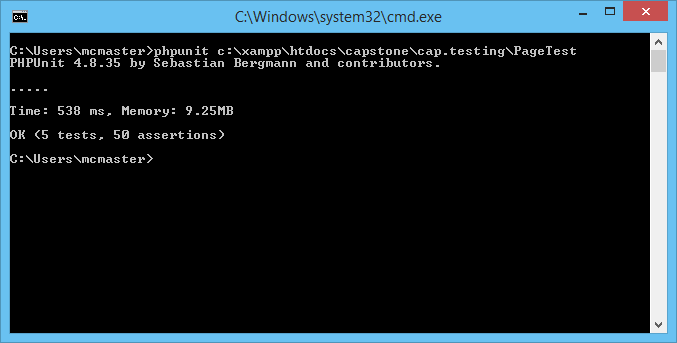
\includegraphics[width=\textwidth,height=\textheight,keepaspectratio]{cmd.png}


\subsection{Traceability}

\subsubsection{Traceability to requirements}

\begin{table}[H]
\caption{Traceability to requirements - System Testing}
\resizebox{\textwidth}{!}{%
\begin{tabular}{|l|l|}
\hline
\textbf{Unit Test} & \textbf{Requirement \#} \\ \hline
testGetInstance() & 1,11,12,13,14 \\ \hline
testGetInstanceByName() & 1,11,12,13,14 \\ \hline
testGetInstanceBySpecial() & 1,11,12,13,14 \\ \hline
testGetRelativeURL() & 1 \\ \hline
testGetURLSafeName() & 1 \\ \hline
\end{tabular}%
}
\end{table}

\subsubsection{Traceability to modules}

\begin{table}[H]
\caption{Traceability to modules - System Testing}
\resizebox{\textwidth}{!}{%
\begin{tabular}{|l|l|}
\hline
\textbf{Unit Test}                  & \textbf{Module}          \\ \hline
testGetInstance()          & Page Management \\ \hline
testGetInstanceByName()    & Page Management \\ \hline
testGetInstanceBySpecial() & Page Management \\ \hline
testGetRelativeURL()       & Page Management \\ \hline
testGetURLSafeName()       & Page Management \\ \hline
\end{tabular}%
}
\end{table}

\subsection{Changes made in response to system tests}

\begin{itemize}

\item A few bugs were discovered and corrected in the Page Management system.

\end{itemize}







\end{document}